\PassOptionsToPackage{unicode=true}{hyperref} % options for packages loaded elsewhere
\PassOptionsToPackage{hyphens}{url}
%
\documentclass[]{article}
\usepackage{lmodern}
\usepackage{setspace}
\setstretch{1.3}
\usepackage{amssymb,amsmath}
\usepackage{ifxetex,ifluatex}
\usepackage{fixltx2e} % provides \textsubscript
\ifnum 0\ifxetex 1\fi\ifluatex 1\fi=0 % if pdftex
  \usepackage[T1]{fontenc}
  \usepackage[utf8]{inputenc}
  \usepackage{textcomp} % provides euro and other symbols
\else % if luatex or xelatex
  \usepackage{unicode-math}
  \defaultfontfeatures{Ligatures=TeX,Scale=MatchLowercase}
\fi
% use upquote if available, for straight quotes in verbatim environments
\IfFileExists{upquote.sty}{\usepackage{upquote}}{}
% use microtype if available
\IfFileExists{microtype.sty}{%
\usepackage[]{microtype}
\UseMicrotypeSet[protrusion]{basicmath} % disable protrusion for tt fonts
}{}
\usepackage{hyperref}
\hypersetup{
            pdfauthor={Apostolos Stamenos \& Tyler Pollard},
            pdfborder={0 0 0},
            breaklinks=true}
\urlstyle{same}  % don't use monospace font for urls
\usepackage[left=1.5cm,right=1.5cm,top=1.5cm,bottom=1.5cm]{geometry}
\usepackage{graphicx,grffile}
\makeatletter
\def\maxwidth{\ifdim\Gin@nat@width>\linewidth\linewidth\else\Gin@nat@width\fi}
\def\maxheight{\ifdim\Gin@nat@height>\textheight\textheight\else\Gin@nat@height\fi}
\makeatother
% Scale images if necessary, so that they will not overflow the page
% margins by default, and it is still possible to overwrite the defaults
% using explicit options in \includegraphics[width, height, ...]{}
\setkeys{Gin}{width=\maxwidth,height=\maxheight,keepaspectratio}
\setlength{\emergencystretch}{3em}  % prevent overfull lines
\providecommand{\tightlist}{%
  \setlength{\itemsep}{0pt}\setlength{\parskip}{0pt}}
\setcounter{secnumdepth}{0}
% Redefines (sub)paragraphs to behave more like sections
\ifx\paragraph\undefined\else
\let\oldparagraph\paragraph
\renewcommand{\paragraph}[1]{\oldparagraph{#1}\mbox{}}
\fi
\ifx\subparagraph\undefined\else
\let\oldsubparagraph\subparagraph
\renewcommand{\subparagraph}[1]{\oldsubparagraph{#1}\mbox{}}
\fi

% set default figure placement to htbp
\makeatletter
\def\fps@figure{htbp}
\makeatother

\usepackage{float}
\usepackage{indentfirst}
\floatplacement{figure}{H}

\title{\vspace{7cm} \LARGE ST502: Final Project}
\author{Apostolos Stamenos \& Tyler Pollard}
\date{4/19/2022}

\begin{document}
\maketitle

\newpage

\section{Part 1}\label{s:part1}

Let \(Y_{i1}, \dots, Y_{in}\) be a simple random sample, where \(i=1\)
denotes that the individual was selected from the population of
nonsmokers and \(i=2\) denotes that the individual was selected from the
population of smokers. For the samples from both population, we assume
the parametric model
\(Y_{i1}, \dots, Y_{in} \overset{\text{iid}}\sim N\left(\mu_i, \sigma_i^2\right)\).

\begin{table}[H]\begin{center}
\caption{{\bf Summary of tests}: .}\label{t:summary}
\begin{tabular}{c|cc|cc|c} \hline
Test & Point Estimate & SE & Test Statistic & p-value & Confidence Interval\\ \hline
Pooled Variance & 0.yyy & 0.0xx & & & \\
Satterthwaite & 0.yyy & 0.0xx & & & \\ \hline
\end{tabular}
\end{center}
\end{table}

\begin{figure}\caption{{\bf yadayadayada}\label{f:hist}}
\centering 
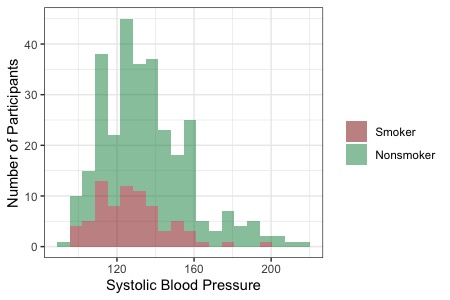
\includegraphics[page=1,width=1.05\textwidth]{hist}
\end{figure}

Both the histograms and the normal QQ plots indicate that the data are
skewed to the right. The boxplots are fairly symmetrical if the outliers
are excluded. We decided to keep the outliers in the analysis. By the
Central Limit Theorem, even if the two datasets are not completely
normal, their sample means are asymptotically normally distributed.
Since the number of smokers and the number of nonsmokers are
sufficiently large, the use of t-tests and confidence intervals are
justified by the Central Limit Theorem.

\begin{figure}\caption{{\bf yadayadayada}\label{f:qq}}
\centering 
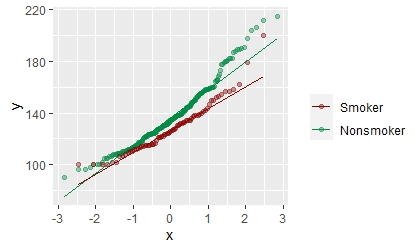
\includegraphics[page=1,width=1.05\textwidth]{qq}
\end{figure}

Both the histograms and the normal QQ plots indicate that the data are
skewed to the right. The boxplots are fairly symmetrical if the outliers
are excluded. We decided to keep the outliers in the analysis. By the
Central Limit Theorem, even if the two datasets are not completely
normal, their sample means are asymptotically normally distributed.
Since the number of smokers and the number of nonsmokers are
sufficiently large, the use of t-tests and confidence intervals are
justified by the Central Limit Theorem.

\begin{figure}\caption{{\bf yadayadayada}\label{f:boxplots}}
\centering 
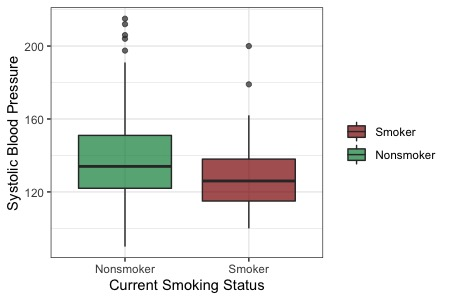
\includegraphics[page=1,width=1.05\textwidth]{boxplots}
\end{figure}

The boxplots indicate that the distribution of systolic blood pressure
for nonsmokers is more spread out than the distribution of systolic
blood pressure for smokers. Based on the boxplots, there is no
indication that the true population variances are equal. To ensure
robustness to the assumption of equal variances, we concluded that the
t-test with the Satterthwaite approximation is preferred.

\section{Part 2}\label{s:part2}

\begin{table}[H]\begin{center}
\caption{{\bf Table of blahblahblahblah}: For most of the scenarios, the power of the xxx test is higher than that for the xxx test.}\label{t:power}
\begin{tabular}{c|cc} \hline
True Parameters & Pooled & Satterthwaite \\ \hline
$\mu_1-\mu_2=$, $n_1=$, $n_2=$, $\sigma_1^2=$, $\sigma_2^2=$ & 0.yyy & 0.0xx  \\
$\mu_1-\mu_2=$, $n_1=$, $n_2=$, $\sigma_1^2=$, $\sigma_2^2=$ & 0.yyy & 0.0xx \\ \hline
\end{tabular}
\end{center}
\end{table}

\end{document}
